% !TEX program = lualatex 
\documentclass[logo, twocolumn]{mlai-report}
\usepackage{url}

\usepackage{titling}

\usepackage[english]{babel}
\usepackage[backend=bibtex8]{biblatex}
\addbibresource{bibliography.bib} 
\usepackage{pifont}
\newcommand{\cmark}{\textcolor[rgb]{0,0.9,0}{\ding{52}}}%
\newcommand{\xmark}{\textcolor[rgb]{0.9,0,0}{\ding{56}}}%

\newcommand{\eg}[2]{ \xmark #1 $\rightarrow$ \cmark #2}

\newif\ifchecklist

\date{} % remove/ fill in to include date

% strange stuff for large page with timeline
\usepackage{rotating}
\usepackage{tikz}
\usepackage{pgfplotstable}
\usetikzlibrary{calc}

\usepackage{hyperref}
\usepackage{cleveref}

\tikzset{>=latex}

\tikzset{
    label/.style=
    {
        minimum width = 3cm,
        text width = 3cm,
        draw=white,
        fill=white
    }
}

\tikzset{
    box/.style=
    {
        rectangle,
        minimum width = 3cm,
        text width = 3cm,
        draw=black,
        fill=white
    }
}

\tikzset{
    round/.style=
    {
        rectangle,
        dashed,
        minimum width = 3cm,
        text width = 3cm,
        draw=black,
        fill=white
    }
}


\title{Student guide for reports and theses at MLAI}

\begin{document}


\maketitle

\begin{abstract}
	This documents collects some guidelines for writing theses, seminar reports, and lab reports within the MLAI group at the University of Bonn.
	Generally, you should ensure that
	the reader always has to know what a section (subsection, paragraph) is about and how it is relevant to the overall context (\textbf{red thread}), that you explain everything in a way such that a colleague of yours would understand it (\textbf{target audience}), that you define everything properly and uniquely and do not contradict yourself (\textbf{inner logic}), that you correctly reference everything that is not your own work (\textbf{no plagiarism}), and that you motivate and explain all choices you made and point out strengths and flaws of your own work (\textbf{critical self-reflection}).

\end{abstract}

\tableofcontents

%\newpage

\section{Initial Remarks}
Writing is a skill that needs to be refined over time. We hope this document will give you a head start, not only by providing best practice advice, but by directing your attention to certain things that will enable you to better reflect on the quality of your document.

\paragraph{Disclaimer} This document is meant as a guide to give you an idea of our expectations regarding written presentation of your results. It can not and does not constitute an exhaustive list of our formal requirements. Thus this document does not provide a base for arguments over grades.

\subsection{Conventions Throughout this Document}
This document collects hints and best practices for scientific writing in general and the various text formats that students have to hand in at our group in particular.
Whenever it is necessary to specify different parameters for different text types, we use the following acronyms:
\begin{description}
\item[BA] Bachelor's thesis
\item[MA] Master's thesis
\item[PG] Projektgruppenbericht
\item[SR] Seminar report
\item[LR] Lab report
\end{description}

\section{Scientific writing in general}
This section contains best practices, tips and tricks on good formal, scientific writing. Presenting your work in an accessible way is as much part of the scientific process as developing methods and conducting experiments. A well structured text reflects sound methodical thinking and makes it easier for the reader to concentrate on the content of your work. \cite{zobel_writing}

% \example{a}{b}
\

\subsection{Language}
\begin{itemize}

	\item Style
	\begin{itemize}
		\item Use present tense (exception: Related Work and parts of Conclusion)
		\item No contractions:
		\begin{center}
			\eg{don't}{do not}\\
			\eg{hasn't}{has not }
		\end{center}
		\item Use active voice \\\eg{the experiments were conducted by X}{X conducted the experiments}
		\item \eg{Sentences spanning multiple lines, especially those that contain many neseted sentences, multiple arguments, many examples and enummerations should be avoided as to not unnecessarily fatigue the reader such that concentrating on the content is as easy at the end of the document as it was in the beginning.}{Avoid sentences that span multiple lines. Convoluted sentence construction is especially tiresome in longer documents.}\\ It is okay to write long sentences initially just to have all your thoughts collected in the document. When subsequently improving this first draft, break down those long sentences into shorter ones so the reader does not get lost.
		\item Choose between British and American English and stay consistent within it.
		\item Use spell checkers
	\end{itemize}
	\item Instead of "I" use "We", as in you, the author, walks the reader through your thinking process.
\end{itemize}

\subsection{Formalia}
\begin{itemize}

	\item The document has to be a \textbf{PDF}.

	\item Length
	\begin{itemize}
		\item PG, SR, LR: 8-10 pages per person required
		\item BA: required are 25-50 pages (we recommend 40)
		\item MA: required are 25-100 pages (we recommend 50)
		\item the pagecount starts with the Introduction (first chapter) and ends with the Conclusion (last chapter)
	\end{itemize}

	\item Citations
	\begin{itemize}
		\item Citations style \textbf{either (Author, year) or [num]}. We recommend the first but chose what fits your style of writing best as long as you stay consistent and don't mix both citation styles.
		\item Citations are placed at the \textbf{end} of the sentence, before the dot ("silent" reference). Exception: "Horv\'ath et al. (2020) have shown \dots" ("loud" reference).\\
		\eg{... by now is a well established fact. [42]}{... by now is a well established fact [42].}
		\item You need to mark \textbf{everything} with a reference that is not part of the current contribution or the current result (i.e. your own work) of this particular document. In particular, referencing your own older work (e.g., a seminar report from last semester) requires a citation. This can include figures (also recreated ones), tables, algorithms, lemmata, results, arguments etc.
	\end{itemize}

	\item Bibliography \label{general_bib}
	\begin{itemize}
		\item Not all types of sources (web pages, proceedings, books) come with the same set of meta data (author, year, edition, date of access, link, chapter, pages) neither is necessarily all the information relevant. Present the information that is necessary for the reader to find the cited source (and perhaps the relevant section) but avoid overloading the entries with redundant or unnecessary information.
		\item Scientific context/ related work: journal article $>$ conference $>$ workshop paper
		\item Basics: textbooks
		\item Misc: web pages
		\item Datasets: Most are associated with a scientific publication. If they are distributed via a website this is also the place where you can usually find information on how to cite them properly.
	\end{itemize}

\end{itemize}

\subsection{Notation and conventions}

\begin{itemize}
	\item Adhere to field specific conventions regarding vocabulary and technical terms, variables and acronyms.
	\item Avoid using ambiguous words (normal, canonical \dots) except when properly introduced beforehand
	\item Definitions should be as formal as possible, a prose explanation of something is good style but only complementary.
	\item Different sources can use the same variable with different meanings. When citing you can adapt those definitions as to avoid ambiguous use for the variables within your document. Stay \textbf{consistent} within your document!
	\item See Section~\ref{sec:helpful-resources}, esp. \cite[pp. 1-8]{knuth_mathematical_writing}
\end{itemize}

\section{Visual Presentation}

In addition to a well structured content a tidy and consistent visual presentation greatly benefits readability. We highly suggest you use \LaTeX.

\subsection{Text}
\begin{itemize}
	\item No headline after a headline
	\item Use a readable font
	\item Font size: 10--12pt
\end{itemize}

\subsection{Non-Text elements}

\begin{itemize}
	\item \LaTeX: \textbf{Floats} \footnote{\href{https://en.wikibooks.org/wiki/LaTeX/Floats,_Figures_and_Captions}{https://en.wikibooks.org/wiki/LaTeX/Floats,\_Figures\_and\_Captions}}
	\begin{itemize}
		\item $\exists \Rightarrow$ use them
		\item Floats wrap around nearly everything that is non-text. They enumerate themselves automatically, can be referenced by name set in $\backslash$label\{\dots\} via $\backslash $ref\{\dots\} and provide a place for a $\backslash$caption\{\dots\}
		\item Each float needs to be referenced and explained in the text
		\item Each float has a caption that gives a standalone explanation
		\item Place floats close to where they are referenced to in the text
	\end{itemize}
	\item Each axis on each plots needs to be labeled
	\item When citing a table from another document, do not use a screen shot bitmap, but instead rebuild the table 
	\item Never use image files such as .png / .jpeg when avoidable. Use \textbf{vector graphics}!
\end{itemize}

\section{Structure of a thesis} \label{sec:structure}

Most theses (and articles, for that matter), are similarly structured. 
A similar structure helps your more seasoned readers (think: examiners) to focus on the content (i.e., what you did). 
It is good to adhere to the standard, everything that distracts the reader from the content that you want to present should be avoided.

Your content and results should be creative, not your layout.
We provide a \LaTeX-template for theses and reports on our homepage.
You may use it as you see fit and change it according to your liking for your thesis.


\begin{enumerate}
	\item Title page
		\begin{itemize}
			\item Title
			\item Name
			\item Date
			\item Supervisor
			\item Examiner(s)
			\item \emph{optional}: Logo of University of Bonn and the MLAI group
		\end{itemize}
	\item Abstract
		\begin{itemize}
			\item BA/MA: max 1 page
			\item Reports: max $\frac{1}{4}$ page
			\item content: what, why, how, results
		\end{itemize}
	\item Acknowledgments/ inspirational quote (optional)
	\item Eigenständigkeitserklärung
	\item Table of content
	\item Lists of Figures, Tables, Abbreviations and Variables (or after bibliography; BA: optional, MA: probably helpful)
	\item Introduction
		\begin{itemize}
			\item cf. Section~\ref{sec:helpful-resources}, esp. \cite{zobel_writing}
			\item motivation
			\item gist of related work
			\item research questions in prose
			\item outline and structure of thesis
		\end{itemize}
	\item Related Work
	\item Preliminaries
		\begin{itemize}
			\item Formally introduce definitions, notation and concepts required to understand the remainder of the document
			\item Target audience: explain everything with as much detail such that a fellow student of yours would be able to understand the document completely. If something was new to you before the thesis: explain it.
			\item You can (and should) give illustrative examples using pictures/ figures to aid comprehension
		\end{itemize}
	\item Main section
		\begin{itemize}
			\item This can span multiple chapters
			\item start with a formal definition of your problem/ research question(s)
			\item describe and motivate your solution; take your time, describe preliminary experiments and trials, visualize examples
			\item how will you solve the problem
			\item why did you chose to do something one way over the other (if two ways are basically equivalent, state this fact and say that you simply preferred doing it this way)
		\end{itemize}
	\item Experiments\\
		Before conduction
		\begin{itemize}
			\item Describe datasets
			\item Setup
			\item What metrics will you report within one experiment (e.g. error or loss) and across experiments (e.g. standard deviation on results)
			\item Baselines/ frames of reference (e.g. other algorithms)
			\item (Briefly) describe all hyper-parameters (of all the methods you use) you had to chose and explain your choice
			\item Explain how your solution will solve the research problem
		\end{itemize} 
		After conduction
		\begin{itemize}
			\item Present the results, if possible visualize them
			\item complete, extensive and objective description of results (this may feel very dry and weird to write at first)
			\item interpret the results
			\item point out expected/ unexpected results
			\item determine whether the results constitute a success regarding the research questions
		\end{itemize}
	\item Conclusion and Future Work
		\begin{itemize}
			\item Summary of thesis
			\item Repeat research question(s)
			\item What was your contribution to solve it
			\item Result of the interpretation
			\item What could be the next steps or further avenues of research from here on?
		\end{itemize}
	\item Bibliography
		\begin{itemize}
			\item See Bibliography in \ref{general_bib}
		\end{itemize}
	\item Appendix
		\begin{itemize}
			\item Additional Figures
			\item lengthy/ detailed proofs
		\end{itemize}
\end{enumerate}

\section{Scopes and scales}

\subsection{Theses}

\paragraph{Bachelor Thesis} \label{Scope BA}
\begin{itemize}
	\item Independent research of literature and interpretation of results. 
	\item Appropriate presentation as a scientific document
	\item Citing mostly text books and only few (proper) papers is okay
\end{itemize}

\paragraph{Master Thesis} \label{Scope MA}
\begin{itemize}
	\item Work autonomously
	\item Considerable length
	\item Solve a significant research problem
	\item Presentation of the research problem and solution within the context of current research
	\item Reflecting knowledge on the current state of the art
	\item Working with primary sources: Papers and the most recent research
	\item Adhere to scientific principles
	\item Demonstrate ability to creatively apply knowledge on the problem at hand
\end{itemize}

\subsection{Reports}

\paragraph{Project Group}
	\begin{itemize}
		\item See BA in \ref{Scope BA} but less content and less literature research
		\item Work together as a group
	\end{itemize}
\paragraph{Seminar Report}
	\begin{itemize}
		\item Summarize and discuss scientific papers autonomously
		\item Summarize content within the context of the seminar
		\item Discuss, analyze and compare content with fellow students and try to see the overall direction of research
	\end{itemize}
\paragraph{Lab Report}
	\begin{itemize}
		\item  MA in \ref{Scope MA} but less content
	\end{itemize}


\section{A Possible Timeline for your Thesis}

It is your task to structure your own work. 
Part of writing a thesis is showing us that you are able to work independently on a scientific topic. 
Hence, we will not force you to do anything or to adhere to any structure that we might feel suitable for a thesis. 
However, Figure~\ref{fig:thesistimeline} provides a generic timeline for your thesis that you might consider as a starting point for your own time table.


% \section{Supervision}

% When writing a thesis or a report, you will have a supervisor who is a member of our group.



\begin{sidewaysfigure}

  \resizebox{\textheight}{!}{
    
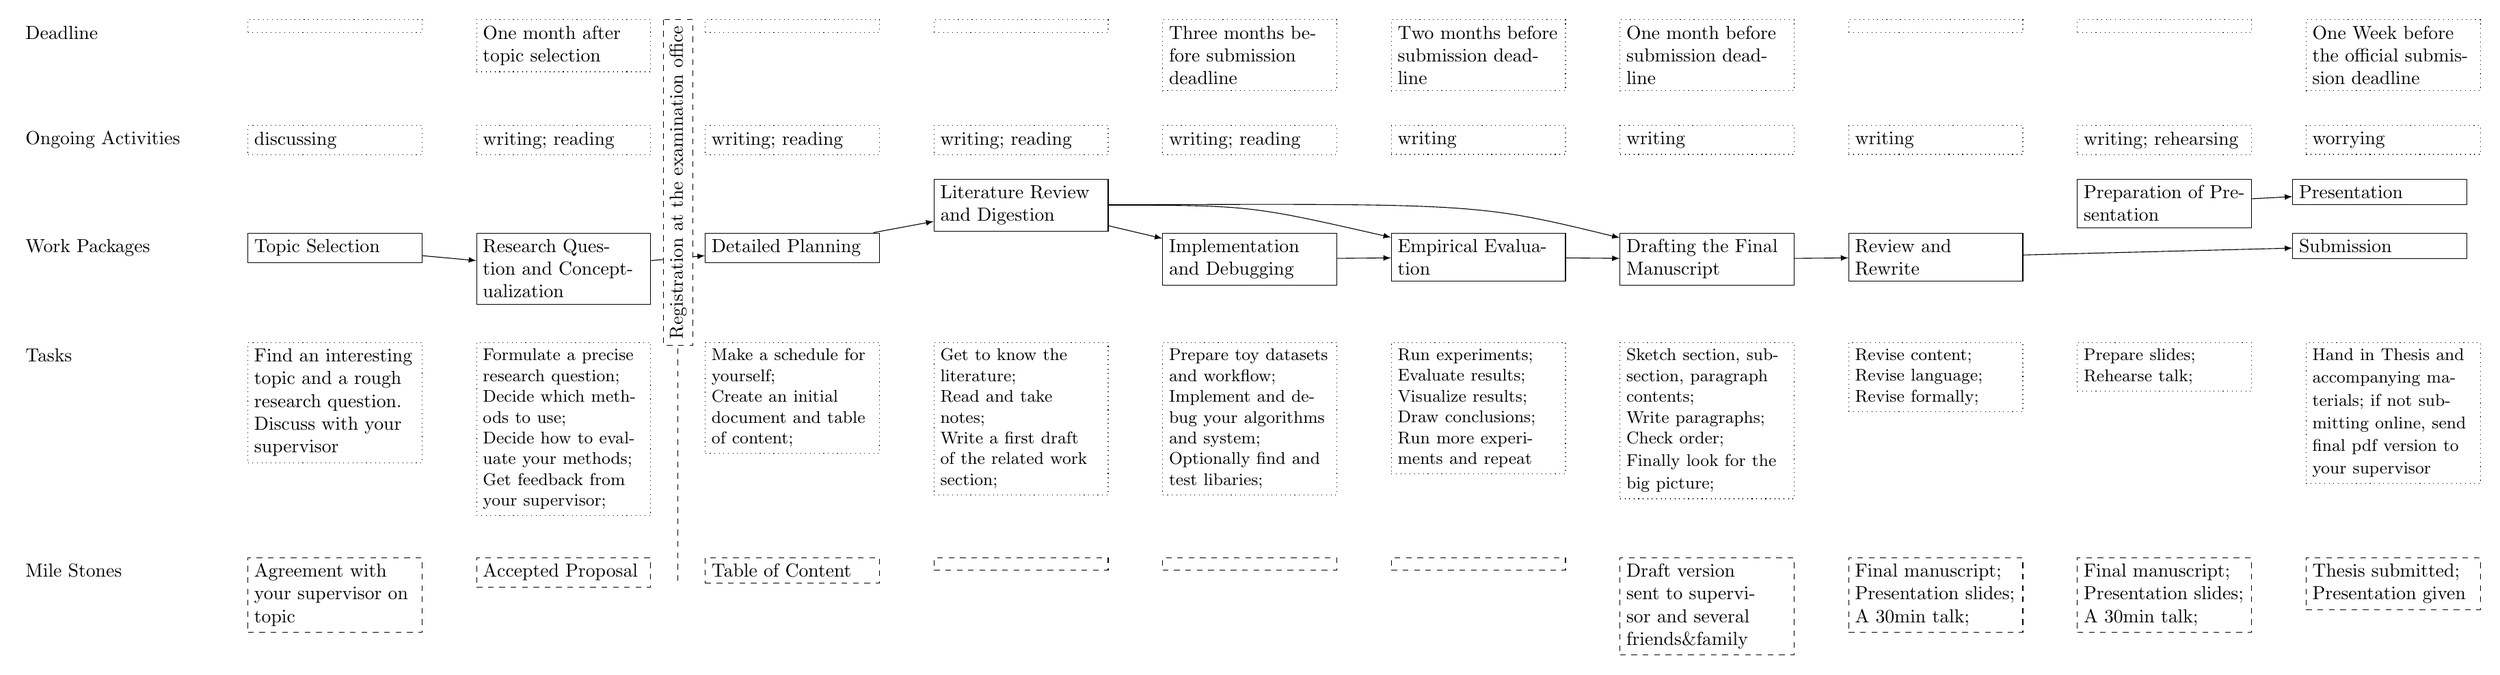
\begin{tikzpicture}
\node[label] (time0) at (0,0) {Deadline};
\node[anchor=west, label] (a0) at ($(time0.west) - (0,2) $) {Ongoing Activities};
\node[anchor=west, label] (m0) at ($(a0.west) - (0,2) $) {Work Packages};
\node[anchor=west, label] (t0) at ($(m0.west) - (0,2) $) {Tasks};
\node[anchor=west, label] (s0) at ($(t0.west) - (0,4) $) {Mile Stones};

\node[anchor=north west, box, dotted] (a1) at ($(a0.north east) + (1,0) $) {discussing};
\node[anchor=north west, box, dotted] (a2) at ($(a1.north east) + (1,0) $) {writing; reading};
\node[anchor=north west, box, dotted] (a3) at ($(a2.north east) + (1,0) $) {writing; reading};
\node[anchor=north west, box, dotted] (a4) at ($(a3.north east) + (1,0) $) {writing; reading};
\node[anchor=north west, box, dotted] (a5) at ($(a4.north east) + (1,0) $) {writing; reading};
\node[anchor=north west, box, dotted] (a6) at ($(a5.north east) + (1,0) $) {writing};
\node[anchor=north west, box, dotted] (a7) at ($(a6.north east) + (1,0) $) {writing};
\node[anchor=north west, box, dotted] (a8) at ($(a7.north east) + (1,0) $) {writing};
\node[anchor=north west, box, dotted] (a8a) at ($(a8.north east) + (1,0) $) {writing; rehearsing};
\node[anchor=north west, box, dotted] (a9) at ($(a8a.north east) + (1,0) $) {worrying};

\node[anchor=north west, box, dotted] (time1) at ($(time0.north east) + (1,0) $) {};
\node[anchor=north west, box, dotted] (time2) at ($(time1.north east) + (1,0) $) {One month after topic selection};
\node[anchor=north west, box, dotted] (time3) at ($(time2.north east) + (1,0) $) {};
\node[anchor=north west, box, dotted] (time4) at ($(time3.north east) + (1,0) $) {};
\node[anchor=north west, box, dotted] (time5) at ($(time4.north east) + (1,0) $) {Three months before submission deadline};
\node[anchor=north west, box, dotted] (time6) at ($(time5.north east) + (1,0) $) {Two months before submission deadline};
\node[anchor=north west, box, dotted] (time7) at ($(time6.north east) + (1,0) $) {One month before submission deadline};
\node[anchor=north west, box, dotted] (time8) at ($(time7.north east) + (1,0) $) {};
\node[anchor=north west, box, dotted] (time8a) at ($(time8.north east) + (1,0) $) {};
\node[anchor=north west, box, dotted] (time9) at ($(time8a.north east) + (1,0) $) {One Week before the official submission deadline};



\node[anchor=north west, box] (m1) at ($(m0.north east) + (1,0) $) {Topic Selection};
\node[anchor=north west, box] (m2) at ($(m1.north east) + (1,0) $) {Research Question and Concept\-ualization};
\node[anchor=north west, box] (m3) at ($(m2.north east) + (1,0) $) {Detailed Planning};
\node[anchor=north west, box] (m4) at ($(m3.north east) + (1,1) $) {Literature Review and Digestion};
\node[anchor=north west, box] (m5) at ($(m4.north east) + (1,-1) $) {Implementa\-tion and Debugging};
\node[anchor=north west, box] (m6) at ($(m5.north east) + (1,0) $) {Empirical Evaluation};
\node[anchor=north west, box] (m7) at ($(m6.north east) + (1,0) $) {Drafting the Final Manuscript};
\node[anchor=north west, box] (m8) at ($(m7.north east) + (1,0) $) {Review and Rewrite};
\node[anchor=north west, box] (m11) at ($(m8.north east) + (1,1) $) {Preparation of Presentation};
\node[anchor=north west, box] (m9) at ($(m8.north east) + (5,0) $) {Submission};
\node[anchor=north west, box] (m10) at ($(m9.north west) + (0,1) $) {Presentation};
\draw[->] (m1) -- (m2); 
\draw[->] (m2) -- (m3); 
\draw[->] (m3) -- (m4); 
\draw[->] (m4) -- (m5); 
\draw[->] (m4) .. controls ($ (m5) + (0,1) $) .. (m6); 
\draw[->] (m4) .. controls ($ (m6) + (0,1) $) .. (m7); 
\draw[->] (m5) -- (m6); 
\draw[->] (m6) -- (m7);
\draw[->] (m7) -- (m8); 
\draw[->] (m8) -- (m9);
\draw[->] (m11) -- (m10);

\node[anchor=north west, box, dotted] (t1) at ($(t0.north east) + (1,0) $) {Find an interesting topic and a rough research question. Discuss with your supervisor};
\node[anchor=north west, box, dotted] (t2) at ($(t1.north east) + (1,0) $) {\small
Formulate a precise research question;\\
Decide which methods to use;\\
Decide how to evaluate your methods;\\
Get feedback from your supervisor;\\
};
\node[anchor=north west, box, dotted] (t3) at ($(t2.north east) + (1,0) $) {\small
Make a schedule for yourself;\\
Create an initial document and table of content;\\
};
\node[anchor=north west, box, dotted] (t4) at ($(t3.north east) + (1,0) $) {\small
Get to know the literature;\\
Read and take notes;\\
Write a first draft of the related work section;\\};
\node[anchor=north west, box, dotted] (t5) at ($(t4.north east) + (1,0) $) {\small
Prepare toy datasets and workflow;\\
Implement and debug your algorithms and system;\\
Optionally find and test libaries;\\
};
\node[anchor=north west, box, dotted] (t6) at ($(t5.north east) + (1,0) $) {\small
Run experiments;\\
Evaluate results;\\
Visualize results;\\
Draw conclusions;\\
Run more experiments and repeat\\
};
\node[anchor=north west, box, dotted] (t7) at ($(t6.north east) + (1,0) $) {\small 
Sketch section, subsection, paragraph contents;\\
Write paragraphs;\\
Check order;\\
Finally look for the big picture;
};
\node[anchor=north west, box, dotted] (t8) at ($(t7.north east) + (1,0) $) {\small
Revise content;\\
Revise language;\\
Revise formally;\\

};
\node[anchor=north west, box, dotted] (t8a) at ($(t8.north east) + (1,0) $) {\small
Prepare slides;\\
Rehearse talk;\\
};
\node[anchor=north west, box, dotted] (t9) at ($(t8a.north east) + (1,0) $) {\small
Hand in Thesis and accompanying materials; 
if not submitting online, send final pdf version to your supervisor};

\node[anchor=north west, round] (s1) at ($(s0.north east) + (1,0) $) {Agreement with your supervisor on topic};
\node[anchor=north west, round] (s2) at ($(s1.north east) + (1,0) $) {Accepted Proposal};
\node[anchor=north west, round] (s3) at ($(s2.north east) + (1,0) $) {Table of Content};
\node[anchor=north west, round] (s4) at ($(s3.north east) + (1,0) $) {};
\node[anchor=north west, round] (s5) at ($(s4.north east) + (1,0) $) {};
\node[anchor=north west, round] (s6) at ($(s5.north east) + (1,0) $) {};
\node[anchor=north west, round] (s7) at ($(s6.north east) + (1,0) $) {Draft version sent to supervisor and several friends\&family};
\node[anchor=north west, round] (s8) at ($(s7.north east) + (1,0) $) {Final manuscript;\\
Presentation slides;\\
A 30min talk;\\};
\node[anchor=north west, round] (s8a) at ($(s8.north east) + (1,0) $) {Final manuscript;\\
Presentation slides;\\
A 30min talk;\\};
\node[anchor=north west, round] (s9) at ($(s8a.north east) + (1,0) $) {Thesis submitted; Presentation given}; 




\coordinate (tn) at (time0.north);
\coordinate (ss) at (s0.south);
\coordinate (start) at ($ (t2.east) + (0.5, 0) $);
\draw[dashed, -] (tn -| start) -- (ss -| start); 
\node [rotate=90, anchor=east, rectangle, dashed, draw=black, fill=white] at (tn -| start) {Registration at the examination office};


\end{tikzpicture}

  }

  \caption{A possible timeline of your thesis.}
  \label{fig:thesistimeline}
\end{sidewaysfigure}



\section{Helpful Resources} \label{sec:helpful-resources} 

Many smart people have written on writing. 
Here are a few references that extend (and probably partially contradict) this compact document.
Feel free to have a look!

\begin{itemize}
       \item \citetitle{keshav_how_to_read} by \textcite{keshav_how_to_read}
       \item \citetitle{zobel_writing} by \textcite{zobel_writing}
       \item \citetitle{knuth_mathematical_writing} by \textcite{knuth_mathematical_writing}
       \item \citetitle{winston_how_to_speak} by \textcite{winston_how_to_speak}
       \item \citetitle{strunkwhite} by \textcite{strunkwhite}
\end{itemize}{}

 % \section{Tooling}
 % \textbf{TODO}
 

% \section{Tooling}
% \textbf{TODO}

\printbibliography

\appendix

%Checkliste ein und ausschalten
\checklisttrue
%\checklistfalse
\ifchecklist 
\newpage
\onecolumn
% student_guide_reporst_theses.tex
\newcounter{formcounter}
\newcommand{\form}{\begin{Form}\ChoiceMenu[name=X\alph{formcounter}, radio,radiosymbol=\ding{52}]{}{ }\end{Form}&\begin{Form}\ChoiceMenu[name=X\alph{formcounter}, radio,radiosymbol=\ding{52}]{}{ }\end{Form}\stepcounter{formcounter}}

\newcommand{\checklistheadline}[1]{%
	\multicolumn{3}{c}{#1}\\\hline
	&ToDo&Done}
\section{Checklist}
\begin{table}[h!]
	\begin{center}
		\renewcommand{\arraystretch}{1.3}
	\begin{tabular}{p{0.75\textwidth}cc}
		\checklistheadline{\textbf{Scientific Writing}}\\
		Work is in present tense (except for Related Work and parts of Conclusion&\form\\
		Active voice  &\form\\
		No contractions in the work&\form\\
		No sentences spanning multiple-lines&\form\\
		The text is consistent, British or American English&\form\\
		The text is spell-checked&\form\\
		
		The length of the work matches the requirements&\form\\
		The citation style is consistent and correct&\form\\
		The bibliography is correct and complete&\form\\
		Every result which is not from this particular document is referenced&\form\\
		
		There is no use ambiguous words &\form\\
		The definitions are formally given &\form\\
		The notation is consistent &\form\\
		\checklistheadline{\textbf{Visual Presentation}}\\
		There is no headline after a headline&\form\\
		The font is readable with font size 10-12pt&\form\\
		\textbf{All} floats have a caption, reference and standalone explanation&\form\\
		\textbf{All} plot axes have labels&\form\\
		There is no screenshot of a table&\form\\
		All graphics are vector graphics or tizpictures&\form\\
		\checklistheadline{\textbf{Structure}}\\
		The work is structured properly, according to \Cref{sec:structure}&\form\\

		
	\end{tabular}	

%		\label{table1}
%		\pgfplotstabletypeset[
%		col sep=comma, string type,
%		columns/column1/.style={
%			column name=\textsc{Task}},
%		columns/column2/.style={
%			column name=\textsc{ToDo}},
%		columns/column3/.style={
%			column name=\textsc{Done}},
%		every head row/.style={
%			after row={\toprule}},
%		every last row/.style={after row=\bottomrule},]{checklisttable.csv} 
	\end{center}
\end{table}
\twocolumn
\else
\fi 
\newpage
\section{List of required Latex packages}
In this sections you can find a list of the packages used for the different templates.

\begin{itemize}
	\item Preable:
	\begin{itemize}
		\item polyglossia
		\item algorithm
		\item algpseudocode
		\item enumitem
		\item csquotes
		\item metalogo
		\item fancyvrb
		\item varioref
		\item hyperref
		\item cleveref
		\item biblatex 
	\end{itemize}
	\item Report and Thesis:
	\begin{itemize}
		\item geometry
		\item translations
		\item xcolor
		\item graphicx
		\item booktabs
		\item mathtools
		\item ntheorem
		\item iftex
		\item inputenc
		\item fontenc
		\item textcomp
		\item tgpagella
		\item fontspec
	\end{itemize}
	\item Thesis:
	\begin{itemize}
		\item fmtcount
		\item emptypage
		\item subcaption
		\item caption
	\end{itemize}
\end{itemize}


\end{document}